\section{Performance Results}
\label{sec:results}

In this section, we present performance results for the MapReduce
graph algorithms of the preceeding section, implemented as small C++
programs calling our MR-MPI library.
The benchmarks were run on a medium-sized Linux cluster made up of 2 GHz
dual-core AMD Opteron processors with a Myrinet network.  Most importantly
for MR-MPI, each node of the cluster has one local disk, which is used
for out-of-core operations in MR-MPI.  To avoid contention for disk I/O, we 
ran all experiments with one MPI process per node.

We ran each of the algorithms on four R-MAT graphs of
different sizes, each on a varying number of processors.  Details of the
input data are shown in Table~\ref{t:rmats}.
The {\it small} problem size (around 8M edges) can typically be used
on a single processor without significant out-of-core operations.
The {\it medium} problem size (around 134M edges) is a 
problem that can be run
on a single processor with out-of-core operations; larger processor 
configurations, however, do not necessarily need out-of-core operations.
The {\it large} problem size (around 2B
edges) requires out-of-core operations and higher processor counts.
%The {\it x-large} problem size
%(around 34B edges) requires most of the machine to run.
All data sets used R-MAT parameters $(a, b, c, d) = (0.57, 0.19, 0.19, 0.05)$.

\begin{table}
\begin{tabular}{|l|c|c|c|c|c|c|c|}
\hline
Data & \# of    & \# of & Maximum \\
Set  & vertices & edges & vertex degree\\
\hline
RMAT-20 (small)   &$2^{20} \approx 1M$ & $2^{23} \approx 8M$ &   \\
RMAT-24 (medium)  &$2^{24} \approx 17M$ & $2^{27} \approx 134M$ &   \\
RMAT-28 (large)   &$2^{28} \approx 268M$ & $2^{31} \approx 2B$&   \\
%RMAT-32 (x-large) &$2^{32} \approx 4B$ & $2^{35} \approx 34B$ &   \\
\hline
\end{tabular}
\caption{Characteristics of R-MAT input data for graph algorithm
experiments.}
\label{t:rmats}
\end{table}

The resulting timings give a sense of the inherent scalability of the
MapReduce algorithms as graph size grows on a fixed number of
processors, and of the parallel scalability for computing on a graph
of fixed size on a growing number of processors.  Where available, we
compare the MapReduce algorithm with other parallel implementations.

\subsection{R-MAT generation results}
Discuss R-MAT generation times.

\subsection{PageRank results}

In Figure~\ref{fig:pr}, we show the performance of the MR-MPI PageRank algorithm
compared to a
distributed-memory matrix-based implementation using the linear
algebra toolkit Trilinos~\cite{Trilinos-Overview} 
and a multi-threaded
implementation
in the Multi-Threaded Graph Library (MTGL)~\cite{MTGL}.
The matrix-based distributed-memory implementation of PageRank
uses Trilinos' Epetra matrix/vector classes to represent the graph and
PageRank vector.
Rows of matrix $A$ and the associated entries of the PageRank vector $x$
are uniquely assigned to processors; a random permutation of the input
matrix achieves processor load balance.
Interprocessor communication gathers $x$ values for matrix-vector
multiplication and sums partial products into the $y$ vector.
Most communication is point-to-point communication,
but some global communication is needed for computing
residuals and norms of $x$ and $y$.
In the multi-threaded MTGL~\cite{MTGL} implementation,
rank propagates via adjacency list traversal
in a compressed sparse-row data structure.
To maintain scalability, code must
be written so that a single thread spawns the loop that processes all
in-neighbors of a given vertex; this detail enables the compiler to generate
hotspot-free code.

Figure~\ref{fig:pr} shows the execution time per PageRank iteration for
R-MAT matrices RMAT-20, RMAT-24 and RMAT-28.  
Converging the PageRank iterations
to tolerance $0.002$ requires five or six iterations.
Several R-MAT matrices of 
each size were generated for the experiments; the average time over the
matrices is reported here.  
The Trilinos implementations show near-perfect
strong scaling for RMAT-20 and RMAT-24.  The MR-MPI 
implementations also demonstrate good strong scaling.  However, MR-MPI's
execution time is at least an order of magnitude greater than the Trilinos
implementation.  This result is due to two factors:  ({\it i}) a 
higher volume of
communication in the MapReduce implementation (where all edges are communicated
in each iteration), compared to the Trilinos implementation (where only
vertex-based data are communicated), and ({\it ii}) out-of-core operations
in MR-MPI were performed because of the page-size restriction, while all
Trilinos operations were performed in-core.  The benefit of MR-MPI's
out-of-core implementation is seen, however, with the RMAT-28 data set, 
which could be solved on smaller processor sets than the Trilinos 
implementation.  For these experiments, the Trilinos implementation required
64 processors for the RMAT-28 data set. 

KDD NOTE:  Need to add XMT results; PBGL would be nice, too.


\begin{figure}[h!]
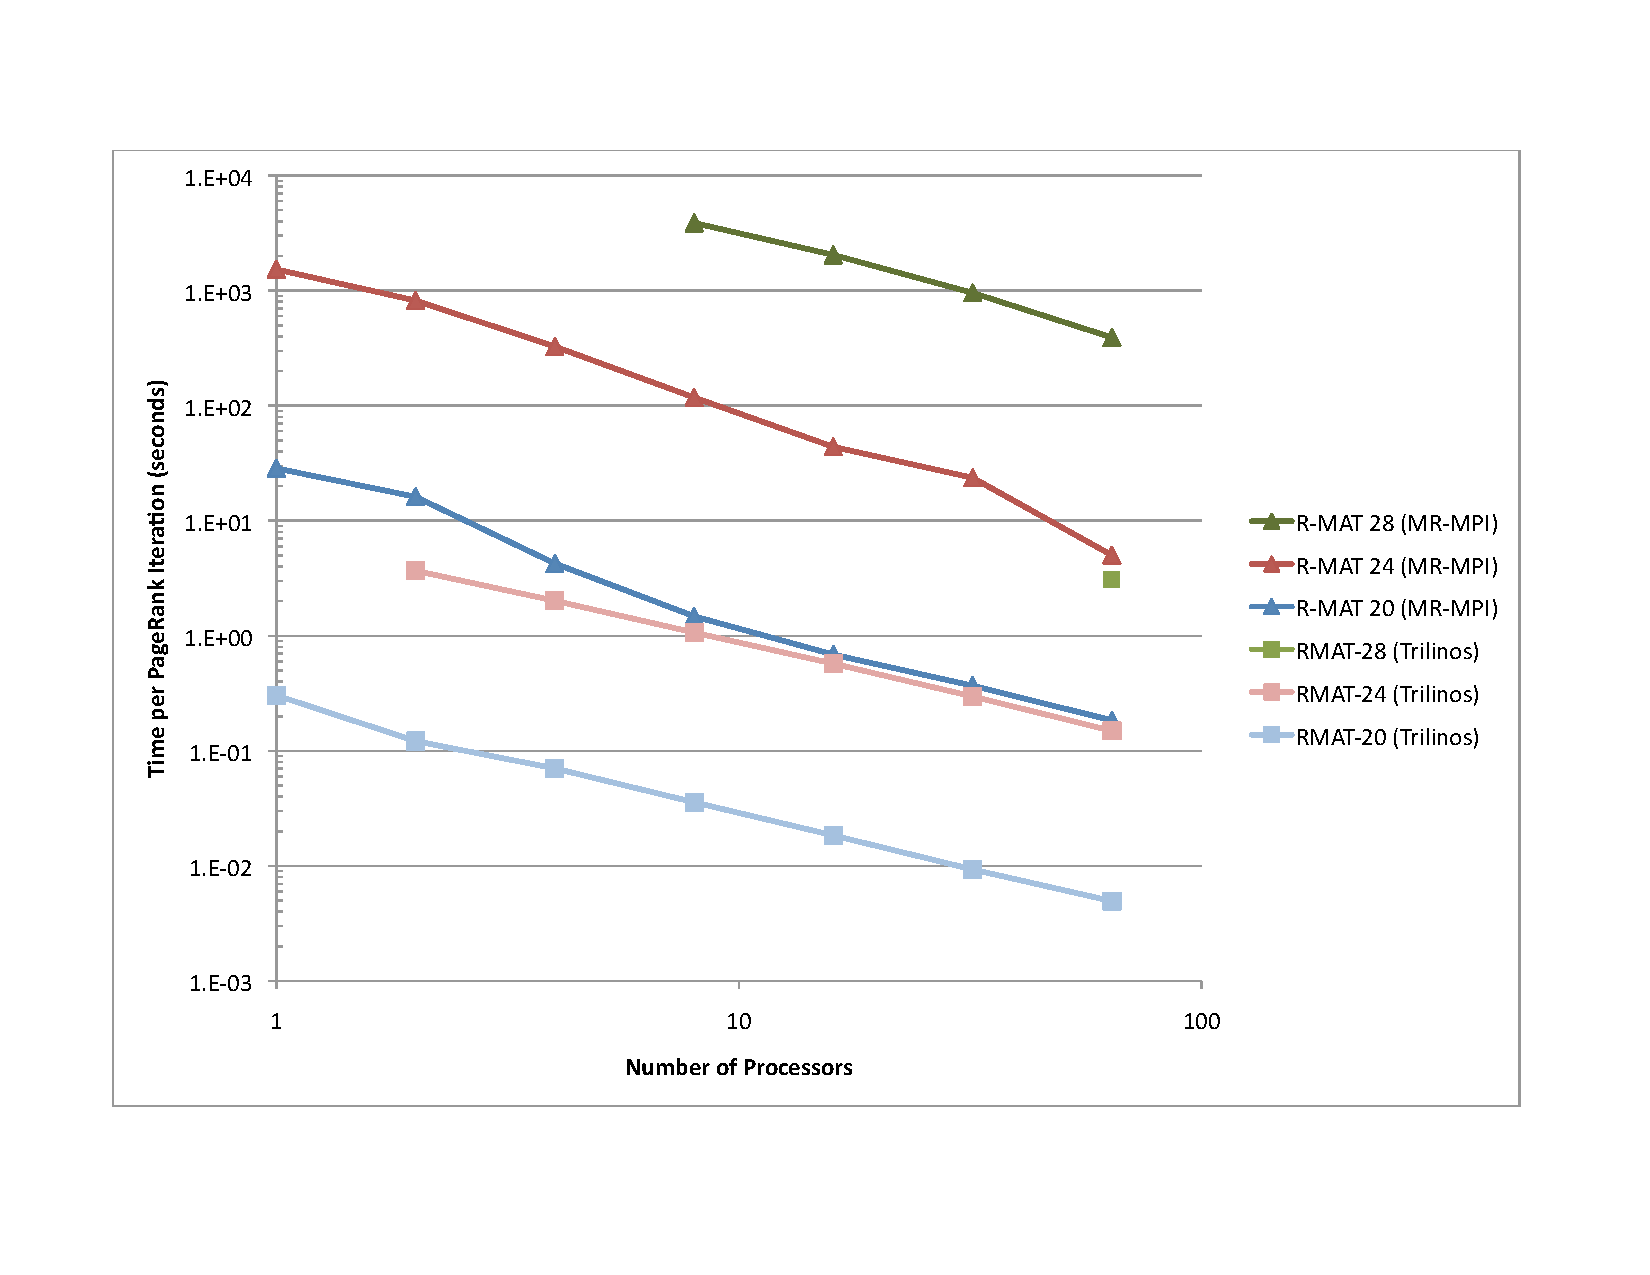
\includegraphics[width=\textwidth]{fig_pagerank.pdf}
\caption{Comparison of PageRank implementations using MapReduce,
Trilinos, and MTGL on R-MAT data sets.}
\label{fig:pr}
\end{figure}



\subsection{Triangle finding results}
Discuss triangle finding times.


\subsection{Maximally independent set results}
Discuss Luby maximally independent sets times.

\subsection{Single-source shortest path results}
Discuss SSSP times.

\subsection{Scalability to large numbers of processors}
Finally, we demonstrate the scalability of MR-MPI to large numbers of 
processors.  
The MR-MPI implementation was run on the Redstorm and Thunderbird
parallel computers
Because these systems do not have local disks for each processor, we selected 
a data set and page sizes that fit in their memory, so out-of-core operations
were not used.  For these experiments, we used an R-MAT data set with 
with $2^{25}$ vertices and $2^{28}$ edges, with parameters given in
Table~\ref{t:rmat}.  We ran both PageRank and Connected Components
algorithms.

\begin{table}
\begin{tabular}{|l|c|c|c|c|c|c|c|}
\hline
Data & R-MAT  & R-MAT  & R-MAT  & R-MAT  & \# of    & \# of & Maximum \\
Set  & a      & b      & c      & d      & vertices & edges & vertex degree\\
\hline
nice  & 0.45 & 0.15 & 0.15 & 0.25 & $2^{25}$ & $2^{28}$ & 1108 \\
nasty & 0.57 & 0.19 & 0.19 & 0.05 & $2^{25}$ & $2^{28}$ & 230,207\\
\hline
\end{tabular}
\caption{Characteristics of R-MAT input data for PageRank and Connected
Components scalability experiments.}
\label{t:rmat}
\end{table}

In Figure~\ref{fig:prbig}, we show the performance 
of the various PageRank
implementations on distributed memory and multi-threaded architectures.
The MR-MPI implementation demonstrated good scalability up to 1024 processors; 
however, it required an order-of-magnitude
more execution time than the matrix-based implementations on Redstorm.  
The distributed memory matrix-based
implementations are competitive with the multi-threaded implementation
in MTGL on the Cray XMT.

\begin{figure}[h!]
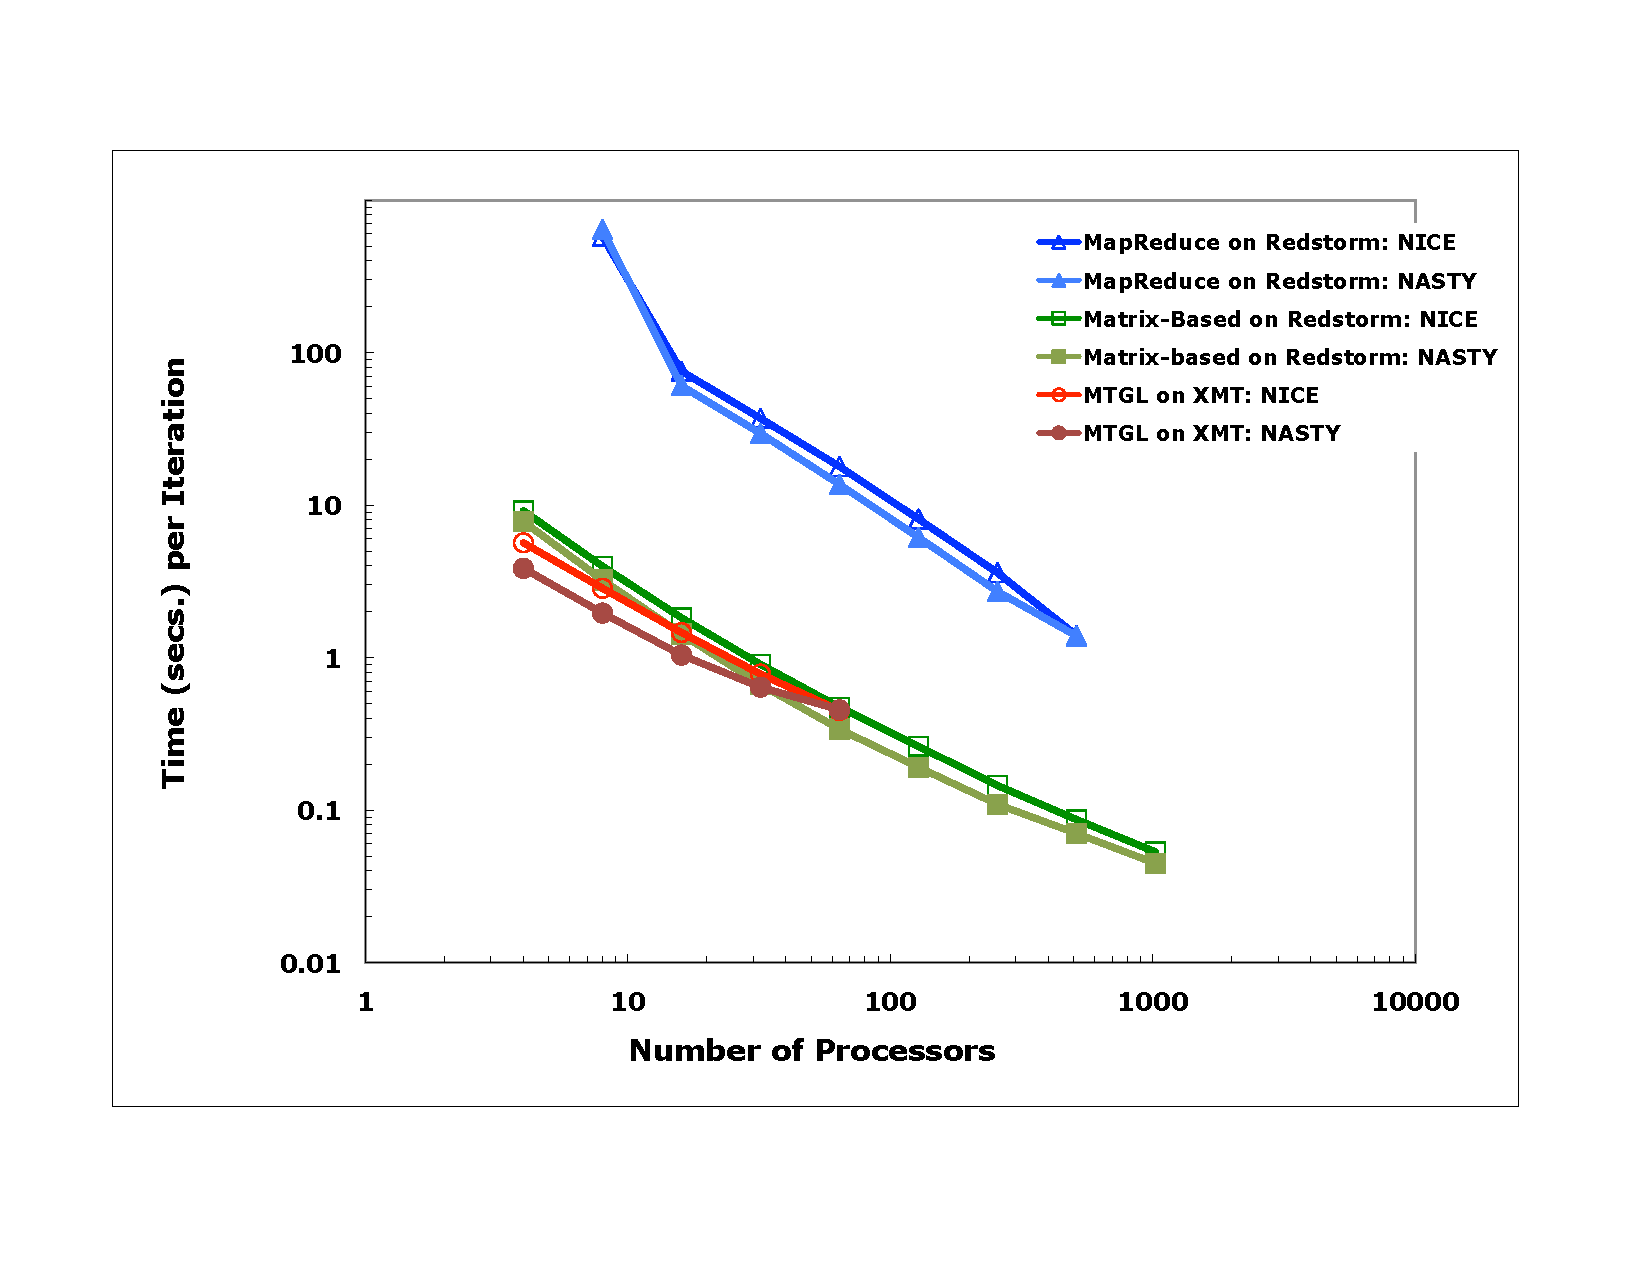
\includegraphics[width=\textwidth]{fig_pagerank_big.pdf}
\caption{Scalability comparison of PageRank implementations using MapReduce,
Trilinos, and MTGL on R-MAT data sets.}
\label{fig:prbig}
\end{figure}

Similar results were obtained for the Connected Components algorithm, as
we show in Figure~\ref{fig:ccbig}.  As with PageRank, the MR-MPI implementation
showed good scalability up to 1024 processors, but required significantly
more time than the Giant Connected Components algorithms using MTGL and
Trilinos.

\begin{figure}[h!]
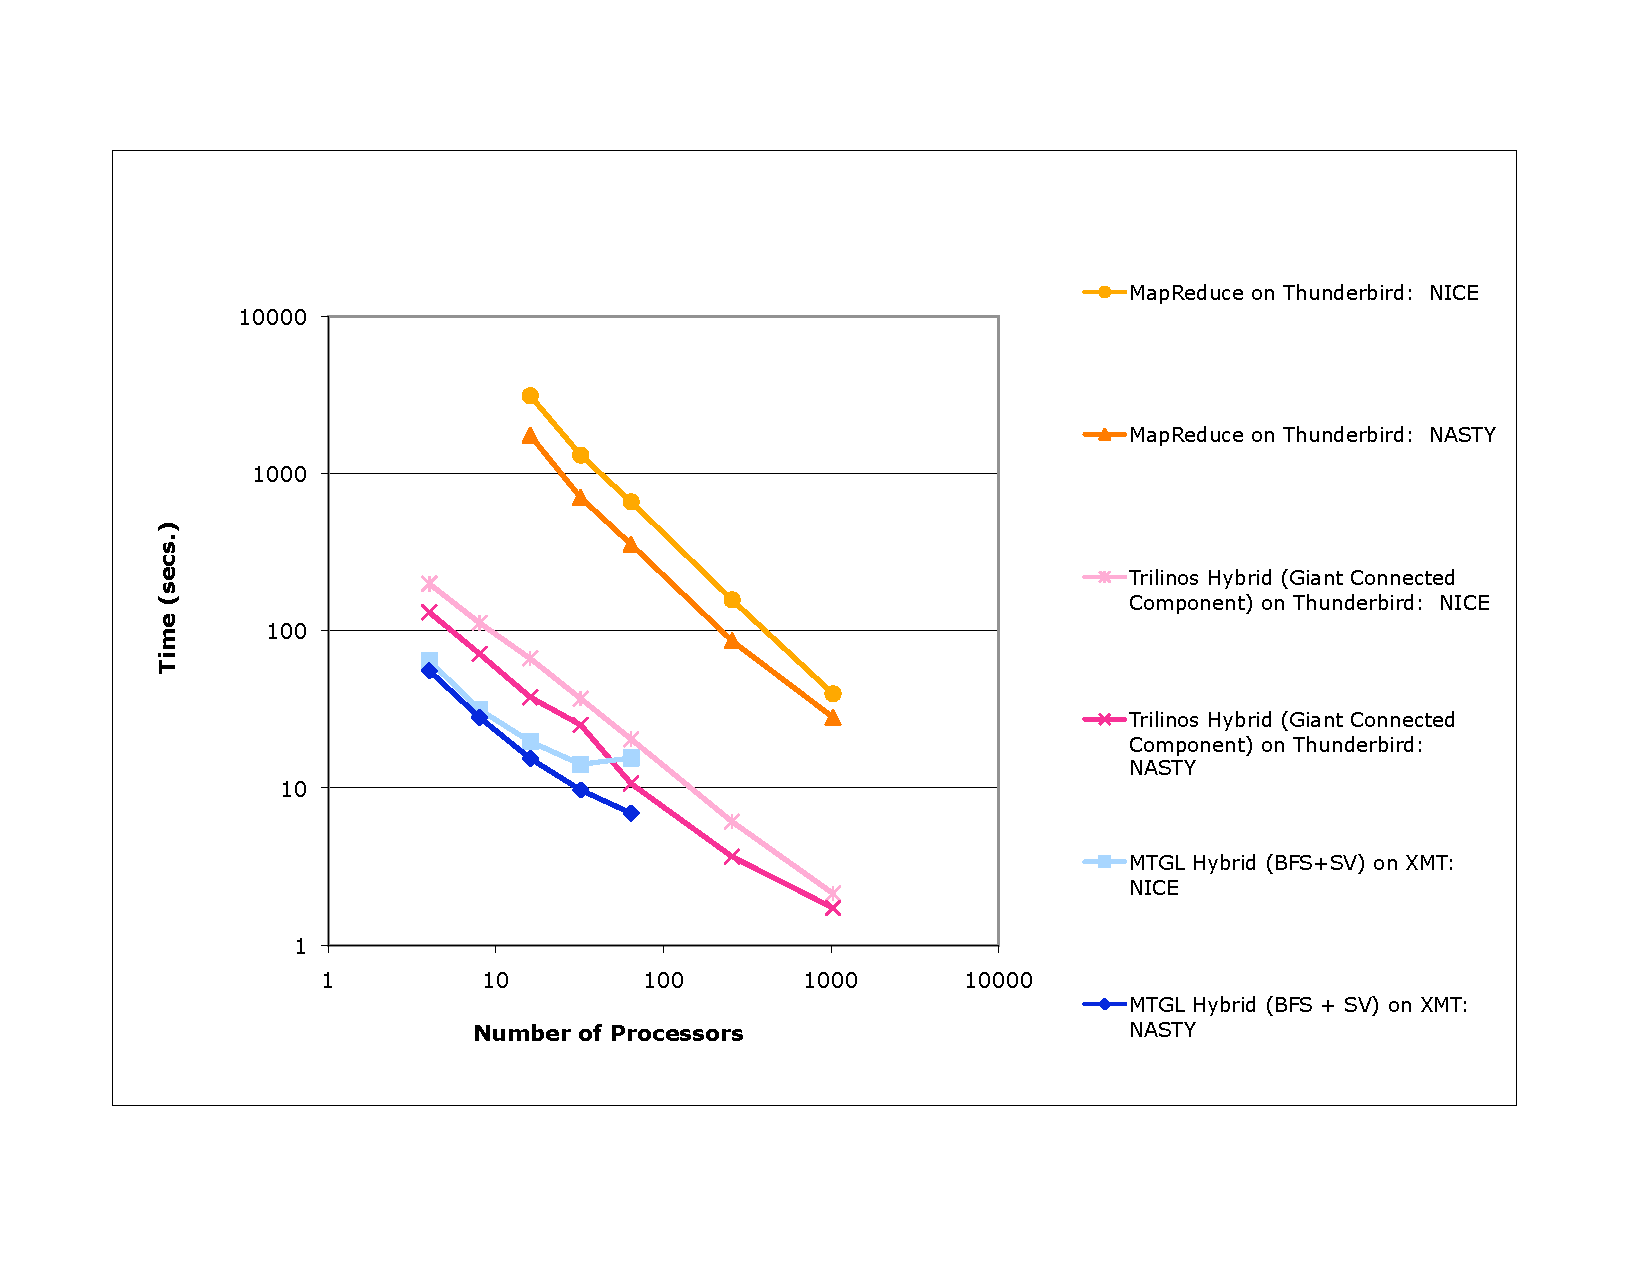
\includegraphics[width=\textwidth]{fig_cc_big.pdf}
\caption{Scalability comparison of Connected Components implementations using MapReduce,
Trilinos, and MTGL on R-MAT data sets.}
\label{fig:ccbig}
\end{figure}

